%<dscrpt>Fichier de déclarations Latex à inclure au début d'un élément de cours.</dscrpt>

\documentclass[a4paper]{article}
\usepackage[hmargin={1.8cm,1.8cm},vmargin={2.4cm,2.4cm},headheight=13.1pt]{geometry}

%includeheadfoot,scale=1.1,centering,hoffset=-0.5cm,
\usepackage[pdftex]{graphicx,color}
\usepackage[french]{babel}
%\selectlanguage{french}
\addto\captionsfrench{
  \def\contentsname{Plan}
}
\usepackage{fancyhdr}
\usepackage{floatflt}
\usepackage{amsmath}
\usepackage{amssymb}
\usepackage{amsthm}
\usepackage{stmaryrd}
%\usepackage{ucs}
\usepackage[utf8]{inputenc}
%\usepackage[latin1]{inputenc}
\usepackage[T1]{fontenc}


\usepackage{titletoc}
%\contentsmargin{2.55em}
\dottedcontents{section}[2.5em]{}{1.8em}{1pc}
\dottedcontents{subsection}[3.5em]{}{1.2em}{1pc}
\dottedcontents{subsubsection}[5em]{}{1em}{1pc}

\usepackage[pdftex,colorlinks={true},urlcolor={blue},pdfauthor={remy Nicolai},bookmarks={true}]{hyperref}
\usepackage{makeidx}

\usepackage{multicol}
\usepackage{multirow}
\usepackage{wrapfig}
\usepackage{array}
\usepackage{subfig}


%\usepackage{tikz}
%\usetikzlibrary{calc, shapes, backgrounds}
%pour la présentation du pseudo-code
% !!!!!!!!!!!!!!      le package n'est pas présent sur le serveur sous fedora 16 !!!!!!!!!!!!!!!!!!!!!!!!
%\usepackage[french,ruled,vlined]{algorithm2e}

%pr{\'e}sentation du compteur de niveau 2 dans les listes
\makeatletter
\renewcommand{\labelenumii}{\theenumii.}
\renewcommand{\thesection}{\Roman{section}.}
\renewcommand{\thesubsection}{\arabic{subsection}.}
\renewcommand{\thesubsubsection}{\arabic{subsubsection}.}
\makeatother


%dimension des pages, en-t{\^e}te et bas de page
%\pdfpagewidth=20cm
%\pdfpageheight=14cm
%   \setlength{\oddsidemargin}{-2cm}
%   \setlength{\voffset}{-1.5cm}
%   \setlength{\textheight}{12cm}
%   \setlength{\textwidth}{25.2cm}
   \columnsep=1cm
   \columnseprule=0.5pt

%En tete et pied de page
\pagestyle{fancy}
\lhead{MPSI-\'Eléments de cours}
\rhead{\today}
%\rhead{25/11/05}
\lfoot{\tiny{Cette création est mise à disposition selon le Contrat\\ Paternité-Pas d'utilisations commerciale-Partage des Conditions Initiales à l'Identique 2.0 France\\ disponible en ligne http://creativecommons.org/licenses/by-nc-sa/2.0/fr/
} }
\rfoot{\tiny{Rémy Nicolai \jobname}}


\newcommand{\baseurl}{http://back.maquisdoc.net/data/cours\_nicolair/}
\newcommand{\urlexo}{http://back.maquisdoc.net/data/exos_nicolair/}
\newcommand{\urlcours}{https://maquisdoc-math.fra1.digitaloceanspaces.com/}

\newcommand{\N}{\mathbb{N}}
\newcommand{\Z}{\mathbb{Z}}
\newcommand{\C}{\mathbb{C}}
\newcommand{\R}{\mathbb{R}}
\newcommand{\D}{\mathbb{D}}
\newcommand{\K}{\mathbf{K}}
\newcommand{\Q}{\mathbb{Q}}
\newcommand{\F}{\mathbf{F}}
\newcommand{\U}{\mathbb{U}}
\newcommand{\p}{\mathbb{P}}


\newcommand{\card}{\mathop{\mathrm{Card}}}
\newcommand{\Id}{\mathop{\mathrm{Id}}}
\newcommand{\Ker}{\mathop{\mathrm{Ker}}}
\newcommand{\Vect}{\mathop{\mathrm{Vect}}}
\newcommand{\cotg}{\mathop{\mathrm{cotan}}}
\newcommand{\sh}{\mathop{\mathrm{sh}}}
\newcommand{\ch}{\mathop{\mathrm{ch}}}
\newcommand{\argsh}{\mathop{\mathrm{argsh}}}
\newcommand{\argch}{\mathop{\mathrm{argch}}}
\newcommand{\tr}{\mathop{\mathrm{tr}}}
\newcommand{\rg}{\mathop{\mathrm{rg}}}
\newcommand{\rang}{\mathop{\mathrm{rg}}}
\newcommand{\Mat}{\mathop{\mathrm{Mat}}}
\newcommand{\MatB}[2]{\mathop{\mathrm{Mat}}_{\mathcal{#1}}\left( #2\right) }
\newcommand{\MatBB}[3]{\mathop{\mathrm{Mat}}_{\mathcal{#1} \mathcal{#2}}\left( #3\right) }
\renewcommand{\Re}{\mathop{\mathrm{Re}}}
\renewcommand{\Im}{\mathop{\mathrm{Im}}}
\renewcommand{\th}{\mathop{\mathrm{th}}}
\newcommand{\repere}{$(O,\overrightarrow{i},\overrightarrow{j},\overrightarrow{k})$}
\newcommand{\cov}{\mathop{\mathrm{Cov}}}

\newcommand{\absolue}[1]{\left| #1 \right|}
\newcommand{\fonc}[5]{#1 : \begin{cases}#2 \rightarrow #3 \\ #4 \mapsto #5 \end{cases}}
\newcommand{\depar}[2]{\dfrac{\partial #1}{\partial #2}}
\newcommand{\norme}[1]{\left\| #1 \right\|}
\newcommand{\se}{\geq}
\newcommand{\ie}{\leq}
\newcommand{\trans}{\mathstrut^t\!}
\newcommand{\val}{\mathop{\mathrm{val}}}
\newcommand{\grad}{\mathop{\overrightarrow{\mathrm{grad}}}}

\newtheorem*{thm}{Théorème}
\newtheorem{thmn}{Théorème}
\newtheorem*{prop}{Proposition}
\newtheorem{propn}{Proposition}
\newtheorem*{pa}{Présentation axiomatique}
\newtheorem*{propdef}{Proposition - Définition}
\newtheorem*{lem}{Lemme}
\newtheorem{lemn}{Lemme}

\theoremstyle{definition}
\newtheorem*{defi}{Définition}
\newtheorem*{nota}{Notation}
\newtheorem*{exple}{Exemple}
\newtheorem*{exples}{Exemples}


\newenvironment{demo}{\renewcommand{\proofname}{Preuve}\begin{proof}}{\end{proof}}
%\renewcommand{\proofname}{Preuve} doit etre après le begin{document} pour fonctionner

\theoremstyle{remark}
\newtheorem*{rem}{Remarque}
\newtheorem*{rems}{Remarques}

\renewcommand{\indexspace}{}
\renewenvironment{theindex}
  {\section*{Index} %\addcontentsline{toc}{section}{\protect\numberline{0.}{Index}}
   \begin{multicols}{2}
    \begin{itemize}}
  {\end{itemize} \end{multicols}}


%pour annuler les commandes beamer
\renewenvironment{frame}{}{}
\newcommand{\frametitle}[1]{}
\newcommand{\framesubtitle}[1]{}

\newcommand{\debutcours}[2]{
  \chead{#1}
  \begin{center}
     \begin{huge}\textbf{#1}\end{huge}
     \begin{Large}\begin{center}Rédaction incomplète. Version #2\end{center}\end{Large}
  \end{center}
  %\section*{Plan et Index}
  %\begin{frame}  commande beamer
  \tableofcontents
  %\end{frame}   commande beamer
  \printindex
}


\makeindex
\begin{document}
\noindent

\debutcours{Approximations des zéros d'une fonction}{alpha}

L'approximation des zéros (ou racines) d'une fonction comporte deux temps : la séparation des racines et l'approximation proprement dite.\newline
La séparation des racines consiste à former des intervalles sur lesquels la restriction de la fonction a de bonnes propriétés et admet une seule racine. Les méthodes proposées ici ne portent que sur les manières de former des valeurs approchées de l'unique zéro dans l'intervalle considéré.\newline
Dans les trois cas, on supposera que la fonction est strictement croissante sur un intervalle $[a,b]$ avec $f(a)<0$ et $f(b)>0$.

\section{Dichotomie}
La méthode de dichotomie repose sur le diagramme suivant et se met en oeuvre très facilement informatiquement. Il est à noter que l'on dispose automatiquement d'une majorations de l'erreur car après $n$ itérations, la racine est entre $a$ et $b$ avec 
\begin{displaymath}
 0<b-a=\frac{b-a}{2^n}
\end{displaymath}
\begin{figure}[ht]
 \centering
 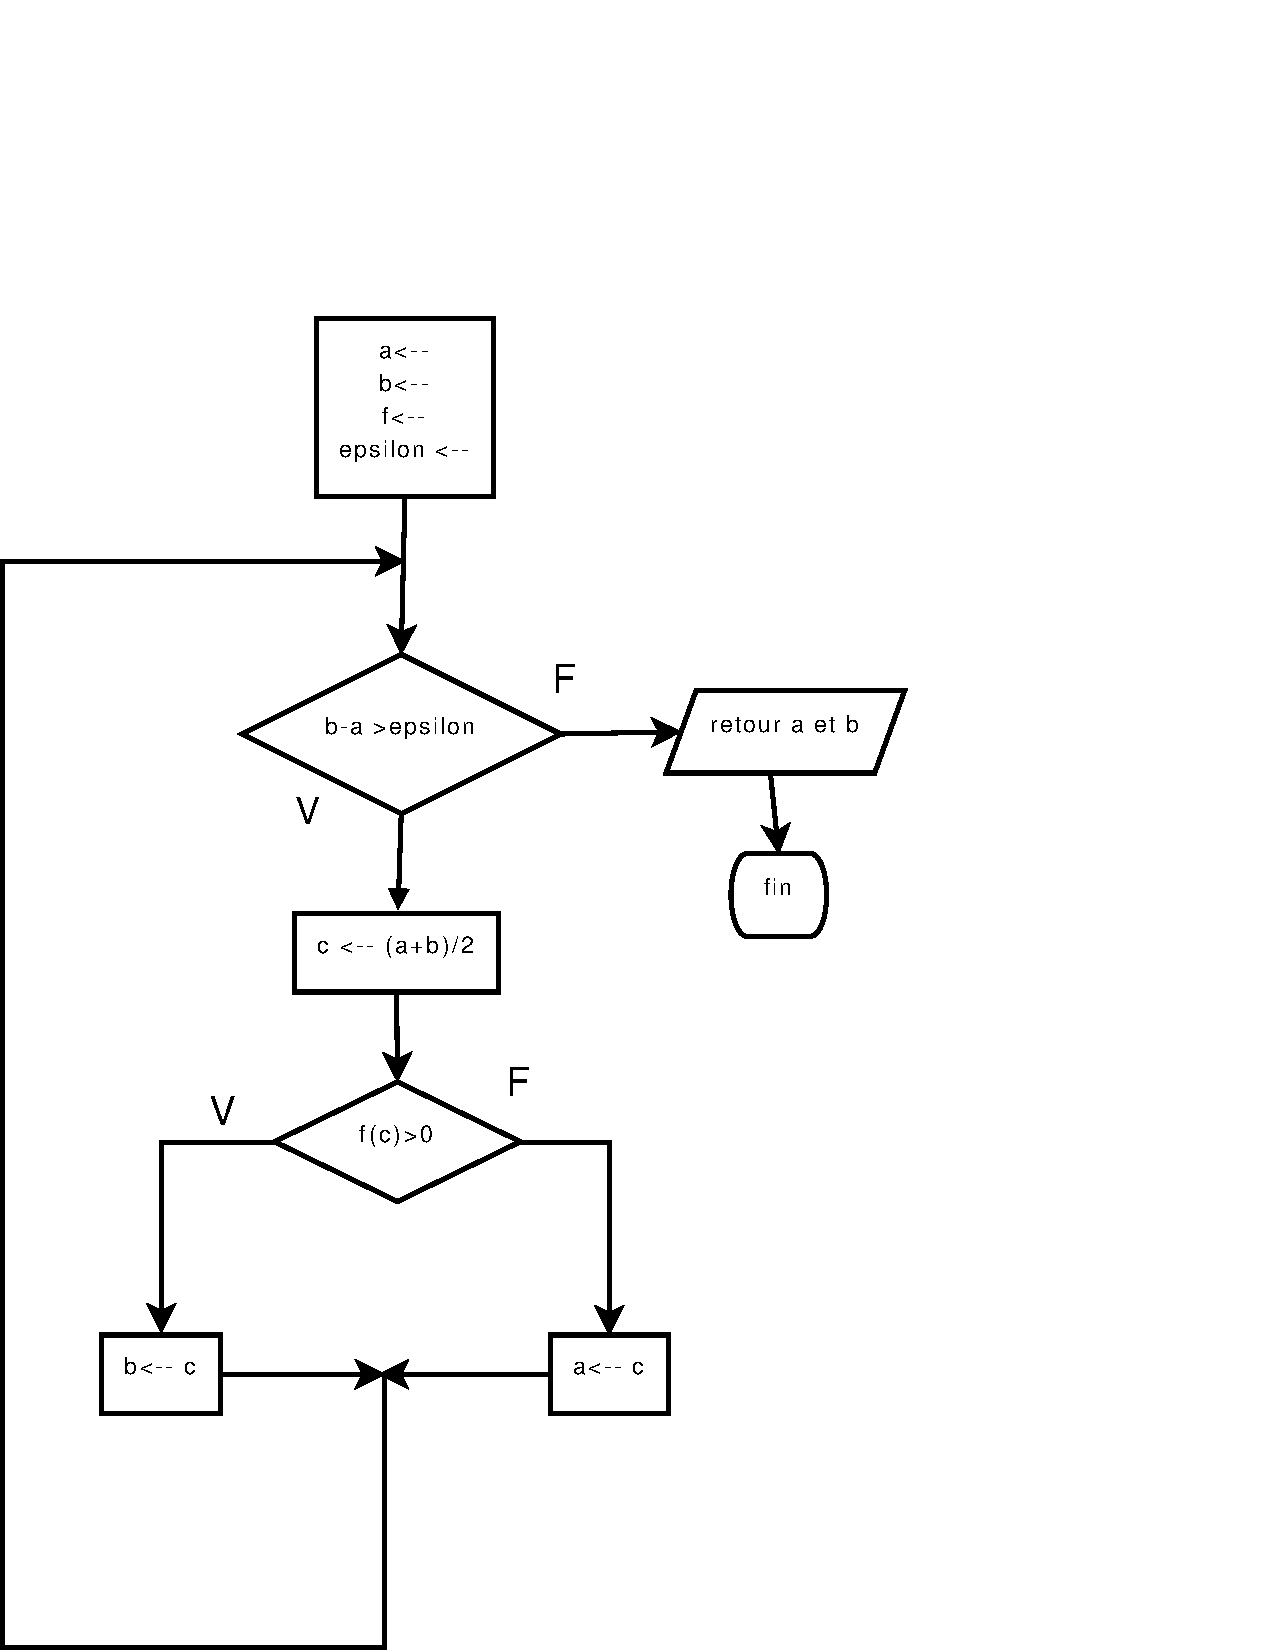
\includegraphics[width=12cm]{C2195_1.pdf}
 \caption{Dichotomie}
\label{C2195_1}
\end{figure}

\section{Méthode de la sécante}
\begin{figure}[ht]
 \centering
\input{C2195_3.pdf_t}
\caption{Méthode de la sécante}
\label{fig:C2195_3}
\end{figure} 
\index{méthode de la sécante}
\index{Interpolation linéaire}

\section{Méthode de Newton}
\begin{figure}[ht]
 \centering
\input{C2195_2.pdf_t}
\caption{Méthode de Newton}
\label{fig:C2195_2}
\end{figure} 
\index{méthode de Newton}
La séparation des racines a conduit à une fonction $f$ de classe $\mathcal C^2([a,b])$ telle que $f(a)<0$, $f(b)>0$, strictement croissante et convexe. L'unique zéro de $f$ est notée $\xi$.\newline
Le principe de la méthode de Newton est de considérer le point d'intersection de la tangente en $M_b$ (de coordonnées $(b,f(b))$ avec l'axe des abscisses. Son abscisse est notée $c$. On démontre alors les résultats suivants :
\begin{displaymath}
 c = b - \frac{f(b)}{f'(b)} \hspace{1cm} \xi < c < b
\end{displaymath}
En effet, un point de coordonnées $(x,y)$ est sur la tangente en $M_b$ si et seulement si
\begin{displaymath}
 y = f(b) +(x-b)f'(b)
\end{displaymath}
On en tire
\begin{displaymath}
 0 = b+ (c-b)f'(b) \Rightarrow c = b - \frac{f(b)}{f'(b)}
\end{displaymath}
Comme $f(b)$ et $f'(b)$ sont strictement positifs, cela prouve aussi $c<b$. Pour l'autre inégalité, on considère l'accroissement entre $\xi$ et $b$, on utilise ensuite le théorème des accroisements finis puis la  croissance de la dérivée:
\begin{displaymath}
 \exists d\in ]\xi,b[ \text{ tel que }
\frac{f(b)}{b-\xi}=\frac{f(b)-f(\xi)}{b-\xi}=f'(d)< f'(b)
\Rightarrow \frac{f(b)}{f'(b)}<b-\xi \Rightarrow \xi < c
\end{displaymath}
On peut donc définir par récurrence une suite $\left(x_n \right)_{n\in\N}$ par :
\begin{displaymath}
 x_0=b\hspace{1cm} x_{n+1} = x_n-\frac{f(x_n)}{f'(x_n)}
\end{displaymath}
D'après les résultats précédents appliqués à un intervalle $[a,x_n]$, cette suite est décroissante et minorée par $\xi$ :
\begin{displaymath}
 \forall n\in \N : \xi < x_{n+1} < x_n
\end{displaymath}
Considérons la fonction $\varphi$ définie par 
\begin{displaymath}
\forall x\in [a,b] : \varphi(x) = -\frac{f(x)}{f'(x)} 
\end{displaymath}
Elle est évidemment continue et vérifie 
\begin{displaymath}
 \varphi(x)=x \Leftrightarrow f(x)=0
\end{displaymath}
On en déduit que la limite de la suite convergente $\left(x_n \right)_{n\in\N}$ est l'unique zéro $\xi$.\newline
En fait cette convergence est très rapide. Cela tient au fait que $\xi$ est un point \og super-attractif \fg de $\varphi$. En effet :
\begin{displaymath}
 \varphi'(x) = \frac{f(x)f''(x)}{f'(x)^2} \Rightarrow \varphi'(\xi)=0
\end{displaymath}
Cela permet d'obtenir des \hyperdef{prop}{major}{formules de majoration d'erreur} très intéressantes et commodes:
\begin{displaymath}
 \left\lbrace 
\begin{aligned}
 0< x_n -\xi \leq&\frac{M_2}{2m_1}(x_{n-1}-x_n)^2\\
 0< x_{n+1}-\xi \leq&\frac{M_2}{2m_1}(\xi-x_n)^2
\end{aligned}
\right. 
\text{ avec } m_1 = \min_{[a,b]}|f'| \text{ et } M_2 = \max_{[a,b]}f'' 
\end{displaymath}
\begin{demo}
 On utilise la formule de Taylor avec reste de Lagrange à l'ordre 2 entre $x_{n-1}$ et $x_{n}$. Il existe $c\in]x_n,x_{n-1}[$ tel que 
\begin{displaymath}
  f(x_{n})=f(x_{n-1})+(x_{n} -x_{n-1})f'(x_{n-1})+\frac{(x_{n}-x_{n-1})^2}{2}f''(c)
\end{displaymath}
Par construction :
\begin{displaymath}
 x_{n}=x_{n-1}-\frac{f(x_{n-1})}{f'(x_{n-1})}\Rightarrow f(x_{n-1)}+ (x_{n} -x_{n-1})f'(x_{n-1})=0
\Rightarrow f(x_{n+1})=\frac{(x_{n+1}-x_{n})^2}{2}f''(c)
\end{displaymath}
D'autre part, en utilisant le théorème des accroissements finis appliqué à $f$ entre $x_{n}$ et $\xi$, il existe $d\in ]\xi,x_{n}[$ tel que 
\begin{displaymath}
 0=f(\xi)=f(x_{n}) + (\xi-x_n)f'(d)
\end{displaymath}
On en déduit
\begin{displaymath}
 x_n -\xi = -\frac{f(x_n)}{f'(d)}= - \frac{(x_{n}-x_{n-1})^2f''(c)}{2f'(d)}\leq \frac{M_2}{2m_1}(x_{n}-x_{n-1})^2
\end{displaymath}
Utilisons maintenant la formule de Taylor avec reste de Lagrange à l'ordre $2$ entre $x_n$ et $\xi$. Il existe $u\in ]\xi,x_n[$ tel que 
\begin{displaymath}
  0=f(\xi)=f(x_{n})+(\xi -x_{n})f'(x_{n})+\frac{(\xi-x_{n})^2}{2}f''(u)
\end{displaymath}
Or
\begin{displaymath}
 x_{n+1} = x_n - \frac{f(x_n)}{f'(x_n)}\Rightarrow f(x_n)-x_nf'(x_n)=-x_{n+1}f'(x_n)
\Rightarrow 0= (\xi -x_{n+1})f'(x_{n})+\frac{(\xi-x_{n})^2}{2}f''(u)
\end{displaymath}
On obtient donc :
\begin{displaymath}
 x_{n+1}-\xi = \frac{(\xi-x_{n})^2f''(u)}{2f'(x_n}\leq \frac{M_2}{2m_1}(\xi-x_{n})^2
\end{displaymath}

\end{demo}
\end{document}
